% ============================================================
% 数电实验报告 — 实验七：基于 FPGA 的模数转换电路
% ============================================================

\documentclass[12pt]{ctexart}

% --- 宏包 ---
\usepackage{graphicx}
\usepackage{amsmath}
\usepackage{xcolor}
\usepackage{float}
\usepackage{booktabs}
\usepackage{siunitx}
\usepackage{fancyhdr}
\usepackage{caption}
\usepackage{subcaption}
\usepackage{hyperref}
\usepackage{makecell}
\usepackage{multirow}
\usepackage{enumitem}
\usepackage{minted}

\sisetup{per-mode=symbol}

\graphicspath{{./figures/}{../figures/}}

\usepackage[left=2.5cm, right=2.5cm, top=2.5cm, bottom=2.5cm]{geometry}

\setlength{\jot}{6pt}
\setlength{\headheight}{15pt}
\linespread{1.5}
\setlist{nosep}

% --- VHDL 代码样式 ---
\setminted[vhdl]{
    fontsize=\small,
    frame=single,
    linenos,
    breaklines,
    tabsize=4,
    numbersep=8pt,
    xleftmargin=2em
}

% --- 页眉页脚 ---
\pagestyle{fancy}
\fancyhead[C]{数字电子技术实验}
\fancyfoot[C]{\thepage}

\begin{document}

% ==================== 封面 ====================
\thispagestyle{empty}

\begin{figure}[t]
    \centering
    
\includegraphics[width=13cm]{logo1.png}
\end{figure}

\vspace*{\fill}
    \begin{center}
        \Huge\textbf{数字电子技术基础}

        \vspace{0.3cm}
        \Huge\textbf{实验报告}

        \vspace{1cm}
        \LARGE\textbf{实验七：基于 FPGA 的模数转换电路}
    \end{center}
\vspace*{\fill}

\begin{table}[H]
    \centering
    \large
    \begin{tabular}{ll}
    \toprule
    \textbf{课程:} & 数字电子技术实验 \\
    \textbf{组员1:} & 郭浩然 2024303980 \\
    \textbf{组员2:} & 庞铭洋 2024302539 \\
    \textbf{组号:} & 15 \\
    \textbf{时间:} & \today \\
    \bottomrule
    \end{tabular}
\end{table}

\newpage

% ==================== 正文 ====================

\section{实验目的}

\begin{enumerate}
    \item 理解高速模数转换芯片 AD9280 的工作原理，掌握它把 $-5\,$V 至 $+5\,$V 模拟电压经衰减后转换成 0 至 255 的 8 位数字码的映射关系。
    \item 掌握用计数器对板载时钟分频的方法，理解为什么要把 50\,MHz 系统时钟分频后才能作为 AD9280 的驱动时钟。
    \item 学会用 VHDL 编写显示译码模块，把 AD 转换得到的特征数据值译码到数码管上显示组员学号，并用 8 位 LED 直接显示数字码。
    \item 熟悉 VHDL 文本设计与原理图设计相结合的混合开发流程，完整走通从建立工程到引脚分配、下载、外接 AD 模块和信号源测试的全过程。
\end{enumerate}

\section{实验要求}

本次实验的要求以现场给出的实验内容为准，具体如下：

\begin{enumerate}
    \item \textbf{要求 1}：用 FPGA 开发板和高速 A/D 模块实现模数转换。用信号源输出频率为 1\,Hz 的方波信号，把方波信号接到 A/D 模块的模拟电压输入端，A/D 模块把模拟信号转换成数字信号。调节信号源幅度旋钮，使输出幅度分别在 $\pm5\,$V、$\pm4\,$V、$\pm3\,$V、$\pm2\,$V、$\pm1\,$V 之间变化，依次记录正负峰值电压对应的 8 位数字输出 \texttt{LED[7..0]}。
    \item \textbf{要求 2}：用信号源产生 1\,Hz 方波，幅度调为 $+5\,$V 至 $-5\,$V 变化。当信号为 $+5\,$V 输出时，两位数码管显示组里一名同学学号的后两位；当信号为 $-5\,$V 输出时，两位数码管显示组里另一名同学学号的后两位；当信号源输出为其他幅度值时，两位数码管显示横线 \texttt{==}。
\end{enumerate}

本组规定：$+5\,$V 时数码管显示郭浩然学号后两位 \texttt{80}，$-5\,$V 时显示庞铭洋学号后两位 \texttt{39}，其他所有输入幅度下两位数码管均显示横线 \texttt{==}，表示当前没有有效的学号显示数据。

\section{实验设备}

\begin{itemize}
    \item DE0-CV 开发板，FPGA 型号为 Cyclone V \texttt{5CEBA4F23C7}
    \item 正点原子高速 AD/DA 子板，模数芯片为 AD9280，8 位 32\,MSPS
    \item 函数信号发生器，提供 1\,Hz 方波并可调幅度
    \item USB-Blaster 下载线及计算机
    \item Quartus II 开发软件
    \item 板载 50\,MHz 晶振、8 位红色 LED、两位七段数码管及连接导线
\end{itemize}

\section{实验原理}

\subsection{AD9280 模数转换原理}

AD9280 是 ADI 公司的一款单芯片 8 位高速模数转换器，最高采样率 32\,MSPS。它在时钟 \texttt{CLK} 的驱动下工作，内置采样保持放大器并采用多级差分流水线结构，从采样到输出数据要经过若干个时钟周期的流水延迟。芯片输出 8 位二进制码，并用 \texttt{OTR} 信号标志输入是否越出量程，量程内为低电平、越界为高电平。

AD9280 本身允许的模拟输入范围是 $0\,$V 至 $2\,$V，对应输出 0 至 255。子板在模拟输入端加了一级衰减电路，把外部 $-5\,$V 至 $+5\,$V 的信号 \texttt{SMA\_IN} 衰减并平移成芯片可接受的 \texttt{AD\_IN2}，二者关系为
\[
    \mathrm{AD\_IN2} = \frac{\mathrm{SMA\_IN}}{5} + 1 .
\]
于是 $\mathrm{SMA\_IN} = -5\,$V 时 $\mathrm{AD\_IN2} = 0\,$V、输出数据 0；$\mathrm{SMA\_IN} = +5\,$V 时 $\mathrm{AD\_IN2} = 2\,$V、输出数据 255。把这两段比例合起来，外部电压 $V$ 与输出数字码 $D$ 之间近似为线性关系
\[
    D = 255 \times \frac{\mathrm{AD\_IN2}}{2}
      = 255 \times \frac{V + 5}{10}
      = 25.5\,(V + 5).
\]
这就是后面用来核对实测数据的理论转换式。

\subsection{时钟分频}

AD9280 支持的最大时钟频率为 32\,MHz，而 DE0-CV 板载系统时钟为 50\,MHz，超过了芯片上限，必须先分频再作驱动时钟。本实验用一个 VHDL 计数器模块 \texttt{freq\_div} 对 50\,MHz 时钟分频，取二分频输出 \texttt{clk\_div\_2} 得到 25\,MHz，接到 AD9280 的 \texttt{ad\_clk} 作为转换驱动时钟，既满足小于 32\,MHz 的限制，又有足够的采样速率跟踪 1\,Hz 的方波。

\subsection{数据显示与译码}

AD 转换得到的 8 位数字码有两条去向。一条直接接到 8 个红色 LED \texttt{D[7..0]}，按二进制逐位点亮，用来直观读出转换结果的数值。另一条接到 VHDL 写的显示译码模块 \texttt{trans}，由它根据特征数据值产生两位数码管的段码，把对应的字符显示出来。译码逻辑见表~\ref{tab:trans}。

\begin{table}[H]
    \centering
    \caption{显示译码模块 trans 的输入数据与数码管显示对照}
    \label{tab:trans}
    \begin{tabular}{cccl}
        \toprule
        \textbf{输入数据 Data\_IN} & \textbf{十进制} & \textbf{对应电压} & \textbf{数码管显示} \\
        \midrule
        \texttt{11111111} & 255 & $+5\,$V 高电位 & \texttt{80}，郭浩然学号后两位 \\
        \texttt{00000000} & 0   & $-5\,$V 低电位 & \texttt{39}，庞铭洋学号后两位 \\
        其他 & 其他 & 其他幅度 & \texttt{==}，无有效数据 \\
        \bottomrule
    \end{tabular}
\end{table}

\subsection{系统结构}

整个系统把文本设计和原理图设计结合起来：分频模块 \texttt{freq\_div} 和译码模块 \texttt{trans} 用 VHDL 编写并各自生成符号，再在顶层原理图中调用并连线。信号流向是：信号源的 1\,Hz 方波接 AD 子板的模拟输入，经衰减电路送 AD9280；FPGA 把 50\,MHz 分频出的 25\,MHz 通过 \texttt{outclk} 引脚送给 AD9280 作驱动时钟；AD9280 转换出的 8 位数据从 GPIO 回到 FPGA 的 \texttt{C[7..0]}，一路直接驱动 8 位 LED，另一路送 \texttt{trans} 译码后驱动两位数码管。顶层原理图见图~\ref{fig:top}。

\begin{figure}[H]
    \centering
    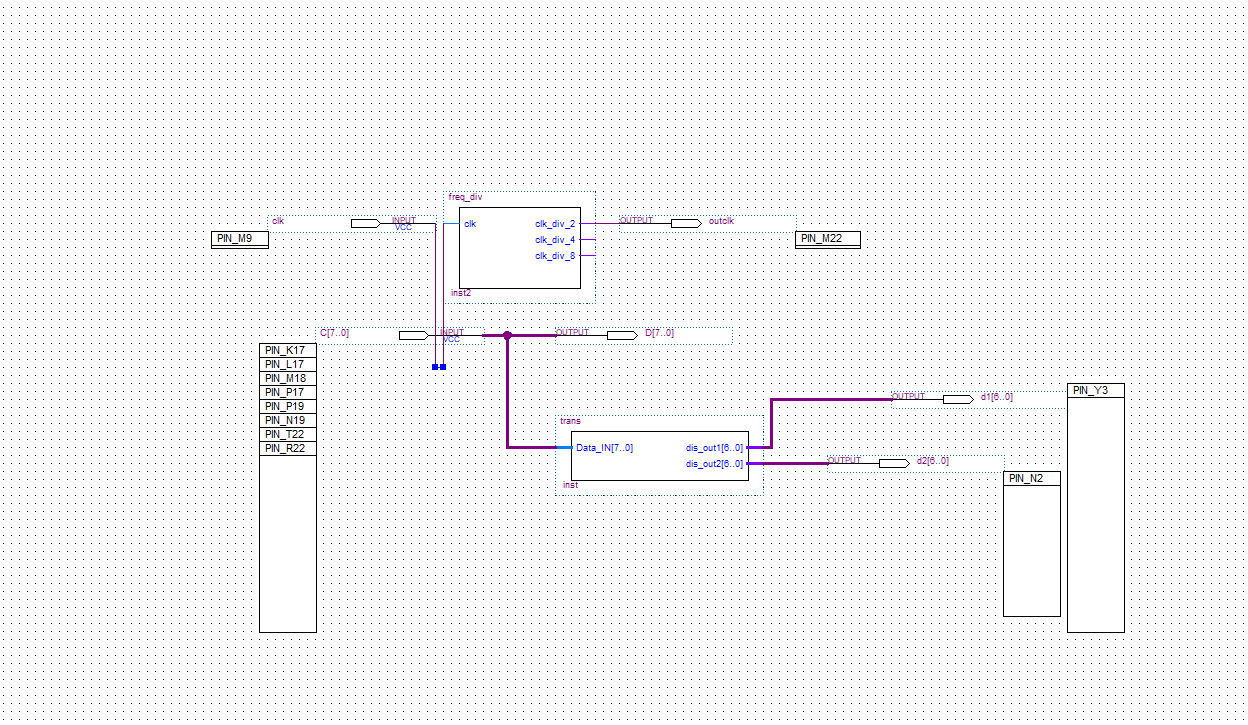
\includegraphics[width=0.95\textwidth]{电路.png}
    \caption{基于 FPGA 的模数转换电路顶层原理图}
    \label{fig:top}
\end{figure}

\section{实验内容}

\subsection{建立工程}

打开 Quartus II，用 \textbf{File $\rightarrow$ New Project Wizard} 新建工程，器件选 DE0-CV 板对应的 Cyclone V \texttt{5CEBA4F23C7}，把顶层实体设为原理图文件 \texttt{top}。随后分别编写两个 VHDL 子模块并绘制顶层原理图。

\subsection{编写分频模块 freq\_div}

\texttt{freq\_div} 用一个 3 位计数器对输入时钟 \texttt{clk} 计数，每个上升沿加 1、计满后归零，再把计数器最低三位分别取反输出 \texttt{clk\_div\_2}、\texttt{clk\_div\_4}、\texttt{clk\_div\_8}，对应二分频、四分频和八分频。本实验取二分频输出 \texttt{clk\_div\_2}，把 50\,MHz 变成 25\,MHz 作 AD9280 的驱动时钟。

\begin{minted}{vhdl}
LIBRARY IEEE;
USE IEEE.STD_LOGIC_1164.ALL;
USE IEEE.STD_LOGIC_ARITH.ALL;
USE IEEE.STD_LOGIC_UNSIGNED.ALL;
ENTITY freq_div IS
PORT (
    clk       : IN  STD_LOGIC;
    clk_div_2 : OUT STD_LOGIC;       -- 二分频，25MHz
    clk_div_4 : OUT STD_LOGIC;       -- 四分频
    clk_div_8 : OUT STD_LOGIC);      -- 八分频
END freq_div;
ARCHITECTURE clk_div_behavior OF freq_div IS
    SIGNAL counter : STD_LOGIC_VECTOR (2 DOWNTO 0);
BEGIN
    PROCESS(clk)
    BEGIN
        IF(clk'EVENT AND clk = '1')THEN
            IF(counter = "111")THEN counter <= "000";
            ELSE counter <= counter + 1;
            END IF;
        END IF;
    END PROCESS;
    clk_div_2 <= NOT counter(0);
    clk_div_4 <= NOT counter(1);
    clk_div_8 <= NOT counter(2);
END clk_div_behavior;
\end{minted}
\captionof{listing}{时钟分频模块 freq\_div.vhd}
\label{lst:freqdiv}

\subsection{编写译码模块 trans}

\texttt{trans} 接收 AD 输出的 8 位数据 \texttt{Data\_IN}，用一段 \texttt{CASE} 组合逻辑把特征值映射成两位数码管的段码 \texttt{dis\_out1}、\texttt{dis\_out2}，实现表~\ref{tab:trans} 的显示。其中 255 显示 \texttt{80}、0 显示 \texttt{39}，其余所有值两位数码管均显示横线 \texttt{==}。

\begin{minted}{vhdl}
library ieee;
use ieee.std_logic_1164.all;
ENTITY trans IS
port (Data_IN  : in  std_logic_vector (7 downto 0);
      dis_out1 : out std_logic_vector (6 downto 0);
      dis_out2 : out std_logic_vector (6 downto 0));
end trans;
ARCHITECTURE fwn OF trans IS BEGIN
PROCESS (Data_IN) BEGIN
CASE Data_IN IS
    WHEN "11111111" => dis_out1 <= "1000000"; dis_out2 <= "0000000"; -- 高电位 80
    WHEN "00000000" => dis_out1 <= "0010000"; dis_out2 <= "0110000"; -- 低电位 39
    WHEN others     => dis_out1 <= "0111110"; dis_out2 <= "0111110"; -- 其他情况显示 ==
END CASE;
END PROCESS;
END fwn;
\end{minted}
\captionof{listing}{显示译码模块 trans.vhd}
\label{lst:trans}

把这两个模块分别编译，再用 \textbf{File $\rightarrow$ Create/Update $\rightarrow$ Create Symbol Files for Current File} 各自生成 \texttt{.bsf} 符号，供顶层原理图调用。

\subsection{绘制顶层原理图}

新建一个 BDF 原理图作为顶层设计，把各模块符号放上去并按下面的关系连线，得到图~\ref{fig:top}。

\begin{itemize}
    \item 输入有两个：\texttt{clk} 接板载 50\,MHz 系统时钟，总线 \texttt{C[7..0]} 接 AD9280 输出的 8 位数据。
    \item \texttt{freq\_div} 以 \texttt{clk} 为输入，二分频输出 \texttt{clk\_div\_2} 接到输出脚 \texttt{outclk}，作为 AD9280 的 25\,MHz 驱动时钟。
    \item 输入总线 \texttt{C[7..0]} 一路直接接输出总线 \texttt{D[7..0]} 驱动 8 位 LED，另一路接 \texttt{trans} 的 \texttt{Data\_IN[7..0]}。
    \item \texttt{trans} 的 \texttt{dis\_out1[6..0]} 接输出 \texttt{d1[6..0]} 驱动第一位数码管，\texttt{dis\_out2[6..0]} 接 \texttt{d2[6..0]} 驱动第二位数码管。
\end{itemize}

\subsection{引脚分配}

把 BDF 设为顶层实体完整编译一遍，再打开 Pin Planner 按表~\ref{tab:pins} 把各端口锁定到 DE0-CV 板和 AD 子板对应的引脚上，引脚配置截图见图~\ref{fig:pin}。其中 \texttt{C[7..0]} 接 GPIO 上 AD 子板的数据口 \texttt{ad\_data[7..0]}，\texttt{outclk} 接 AD 子板的 \texttt{ad\_clk}。

\begin{table}[H]
    \centering
    \caption{引脚分配：端口与 DE0-CV 板载资源及 AD 模块的对应关系}
    \label{tab:pins}
    \begin{tabular}{llll}
        \toprule
        \textbf{端口} & \textbf{方向} & \textbf{引脚} & \textbf{说明} \\
        \midrule
        \texttt{clk}      & 输入 & \texttt{PIN\_M9} & 板载 50\,MHz 系统时钟 \\
        \texttt{C[7..0]}  & 输入 & \texttt{K17,L17,M18,P17,P19,N19,T22,R22} & AD9280 数据 \texttt{ad\_data[7..0]} \\
        \texttt{outclk}   & 输出 & \texttt{PIN\_M22} & 25\,MHz 时钟，接 AD \texttt{ad\_clk} \\
        \texttt{D[7..0]}  & 输出 & \texttt{W2,Y3,N2,N1,U2,U1,L2,L1} & 8 位 LED，显示 AD 数据 \\
        \texttt{d1[6..0]} & 输出 & \texttt{U21,V21,W22,W21,Y22,Y21,AA22} & 第一位数码管 HEX0 \\
        \texttt{d2[6..0]} & 输出 & \texttt{AA20,AB20,AA19,AA18,AB18,AA17,U22} & 第二位数码管 HEX1 \\
        \bottomrule
    \end{tabular}
\end{table}

\begin{figure}[H]
    \centering
    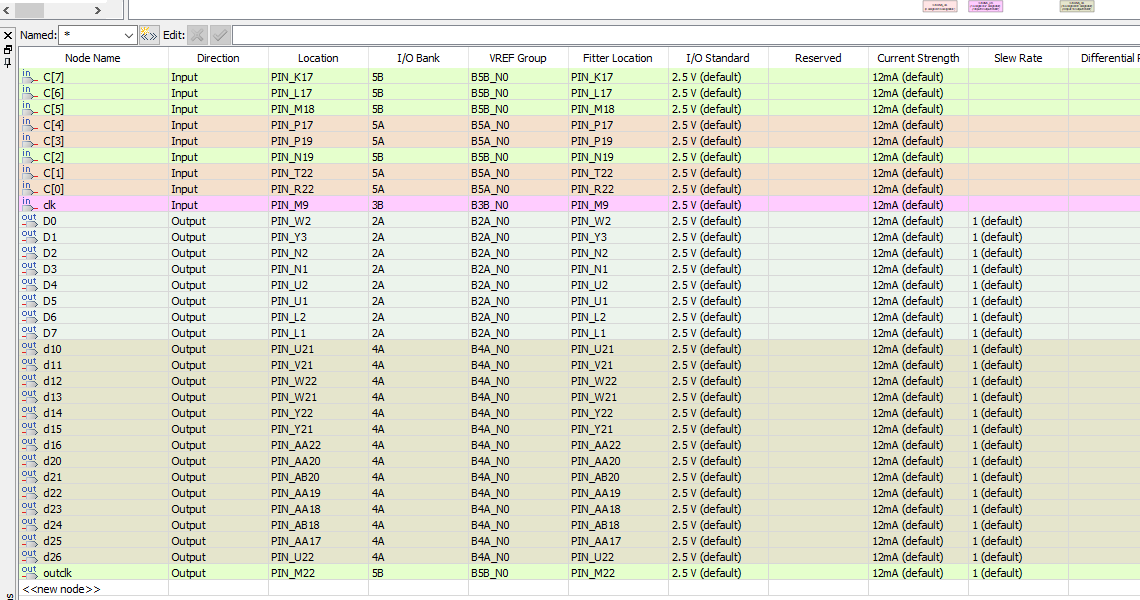
\includegraphics[width=0.95\textwidth]{引脚配置.png}
    \caption{Pin Planner 引脚分配截图}
    \label{fig:pin}
\end{figure}

\subsection{编译与下载}

重新完整编译生成 \texttt{.sof} 配置文件，接上 USB-Blaster，用 JTAG 模式把配置文件下载到 DE0-CV 开发板。

\subsection{接线与测试}

把函数信号源的输出接到 AD 子板的模拟输入端 \texttt{SMA\_IN}，AD 子板的 8 位数据口和 \texttt{ad\_clk} 通过排针接到 FPGA 对应的 GPIO。信号源设为 1\,Hz 方波，先把幅度调到 $\pm5\,$V，再依次减到 $\pm4\,$V、$\pm3\,$V、$\pm2\,$V、$\pm1\,$V，每一档分别在方波的正峰和负峰读出 8 位 LED 显示的二进制数字码，同时观察两位数码管的显示。

\subsection{实验数据}

各档幅度下正负峰电压对应的 8 位数字输出实测值见表~\ref{tab:data}，原始记录见图~\ref{fig:rawdata}。方波幅度为 $\pm5\,$V 时，正峰和负峰对应的数码管显示和 LED 状态见图~\ref{fig:disp} 的 (a) 和 (b)；其他输入幅度下数码管显示横线 \texttt{==}，见图~\ref{fig:disp} 的 (c)。

\begin{table}[H]
    \centering
    \caption{各档幅度下正负峰电压的 8 位数字输出实测值}
    \label{tab:data}
    \begin{tabular}{ccccc}
        \toprule
        \textbf{信号源幅度} & \textbf{峰值电压} & \textbf{LED[7..0] 二进制} & \textbf{十进制} \\
        \midrule
        \multirow{2}{*}{$\pm5\,$V} & $+5\,$V & \texttt{11111111} & 255 \\
                                   & $-5\,$V & \texttt{00000000} & 0   \\
        \midrule
        \multirow{2}{*}{$\pm4\,$V} & $+4\,$V & \texttt{11101111} & 239 \\
                                   & $-4\,$V & \texttt{00010111} & 23  \\
        \midrule
        \multirow{2}{*}{$\pm3\,$V} & $+3\,$V & \texttt{11001101} & 205 \\
                                   & $-3\,$V & \texttt{00110001} & 49  \\
        \midrule
        \multirow{2}{*}{$\pm2\,$V} & $+2\,$V & \texttt{10110011} & 179 \\
                                   & $-2\,$V & \texttt{01001011} & 75  \\
        \midrule
        \multirow{2}{*}{$\pm1\,$V} & $+1\,$V & \texttt{10011001} & 153 \\
                                   & $-1\,$V & \texttt{01100101} & 101 \\
        \bottomrule
    \end{tabular}
\end{table}

\begin{figure}[H]
    \centering
    
\includegraphics[width=0.7\textwidth]{数据.jpg}
    \caption{8 位数字输出原始记录}
    \label{fig:rawdata}
\end{figure}

\begin{figure}[H]
    \centering
    \begin{subfigure}{0.48\textwidth}
        \centering
        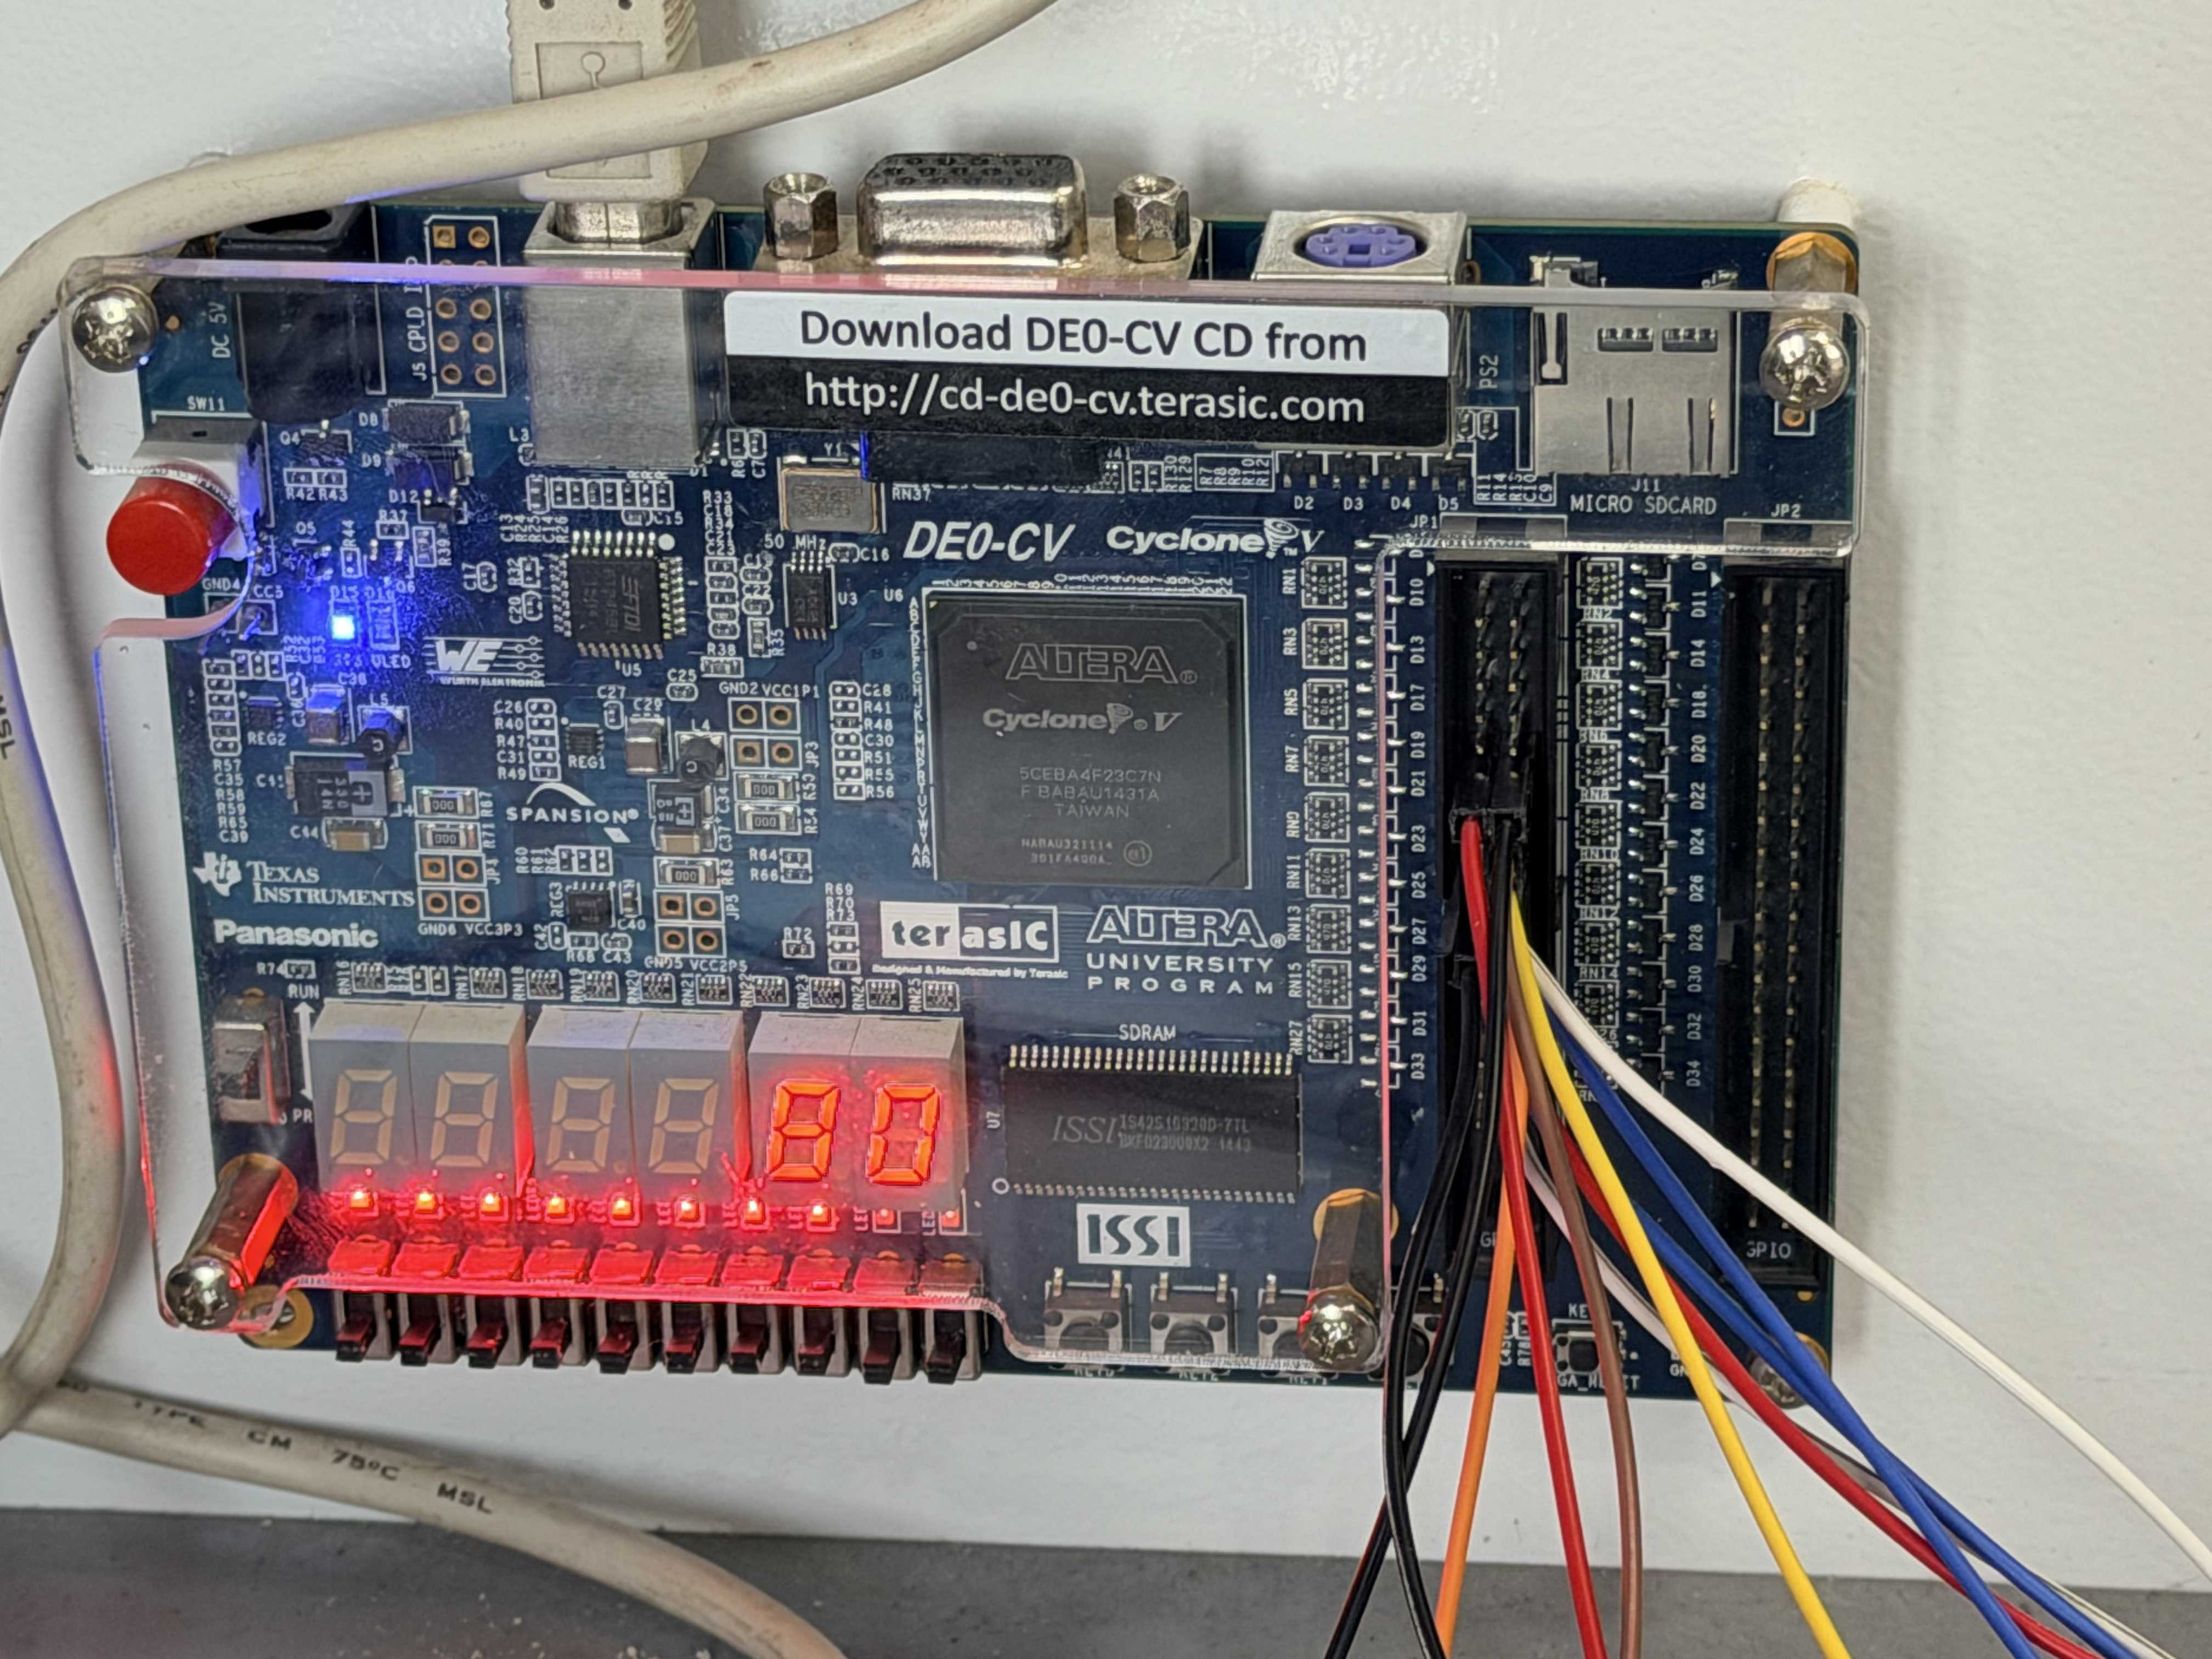
\includegraphics[width=\linewidth]{80.jpg}
        \caption{$+5\,$V，数码管显示 80，LED 全亮}
    \end{subfigure}\hfill
    \begin{subfigure}{0.48\textwidth}
        \centering
        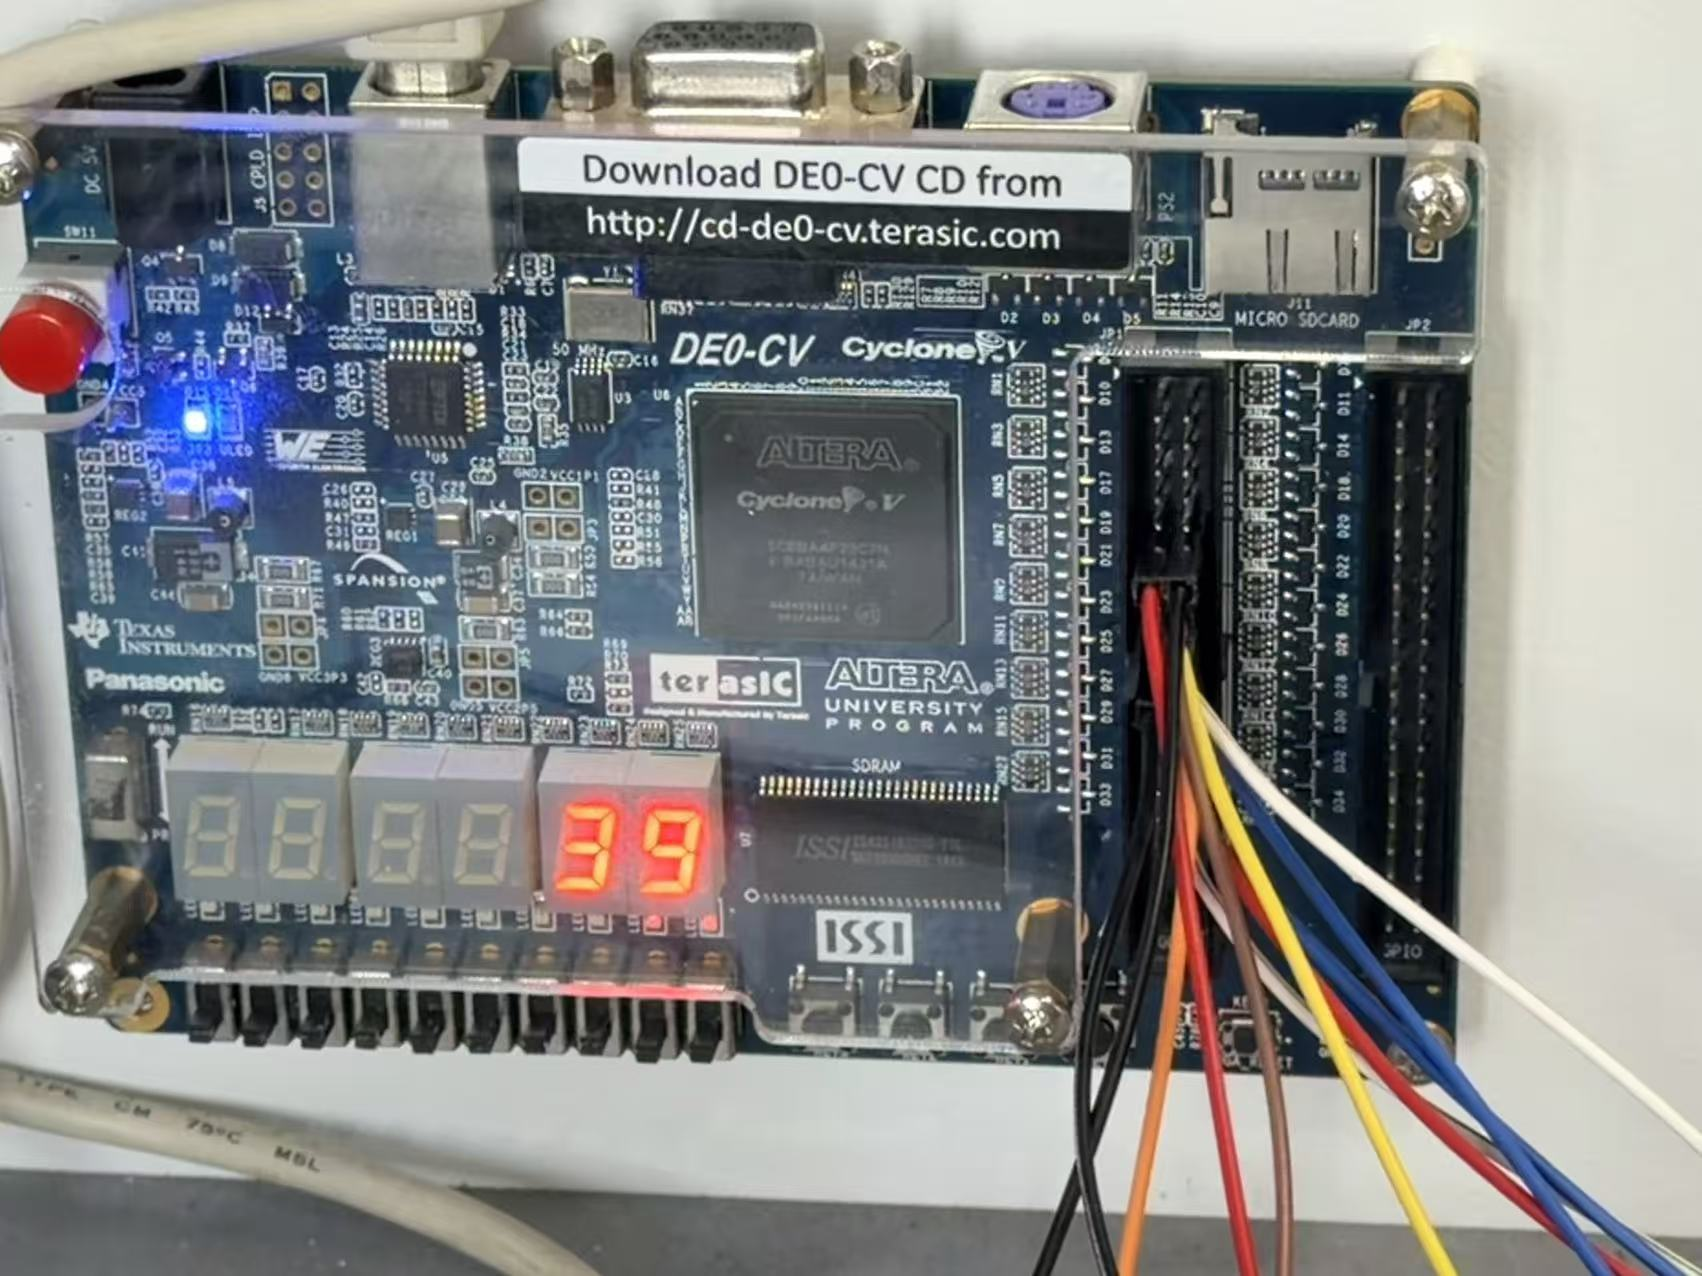
\includegraphics[width=\linewidth]{39.jpg}
        \caption{$-5\,$V，数码管显示 39，LED 全灭}
    \end{subfigure}

    \vspace{6pt}
    \begin{subfigure}{0.6\textwidth}
        \centering
        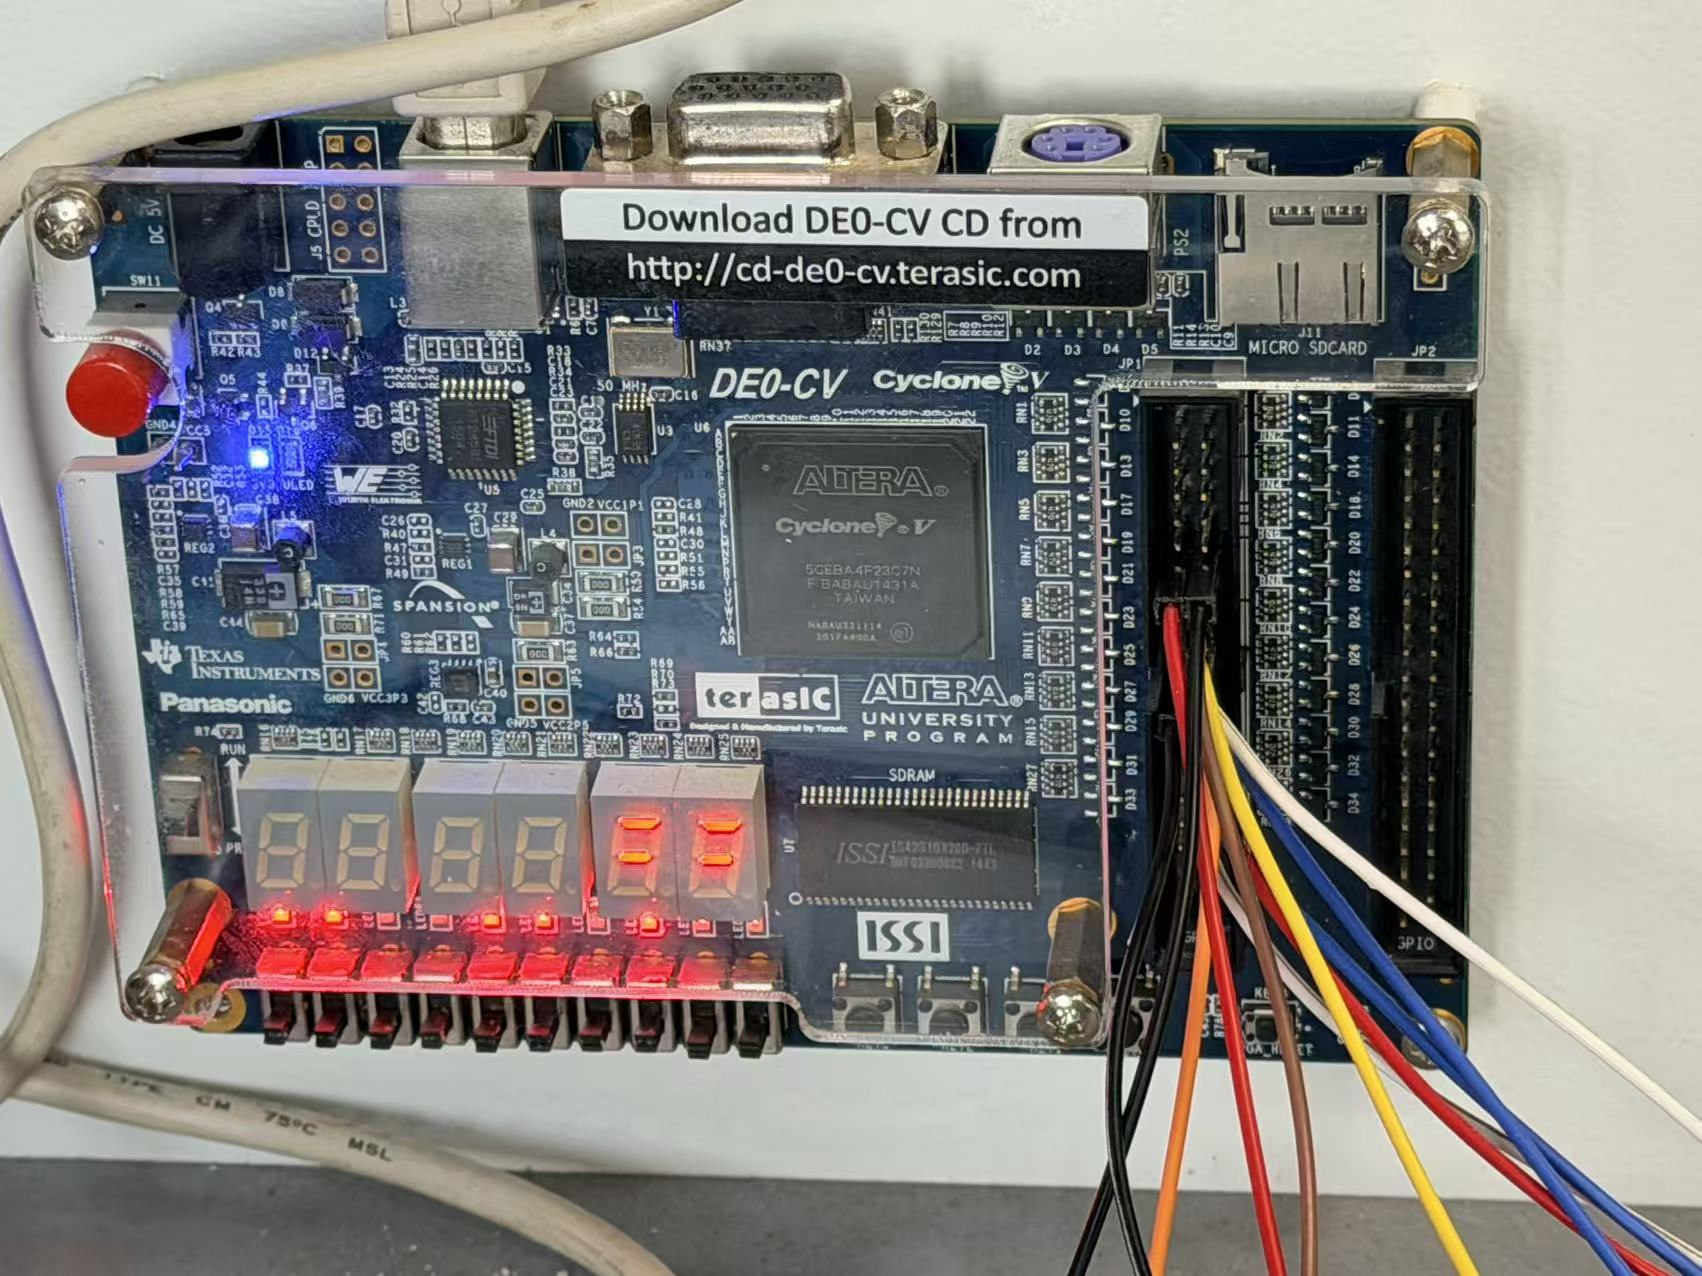
\includegraphics[width=\linewidth]{==.jpg}
        \caption{其他幅度值，数码管显示 \texttt{==}}
    \end{subfigure}
    \caption{两位数码管显示的实测结果}
    \label{fig:disp}
\end{figure}

\subsection{数据分析}

按理论转换式 $D = 25.5\,(V + 5)$ 算出各电压对应的理论数字码，与实测值对照并计算误差，见表~\ref{tab:compare}。

\begin{table}[H]
    \centering
    \caption{实测数字码与理论值对照}
    \label{tab:compare}
    \begin{tabular}{cccc}
        \toprule
        \textbf{峰值电压} & \textbf{理论值} & \textbf{实测值} & \textbf{误差} \\
        \midrule
        $+5\,$V & 255 & 255 & 0   \\
        $-5\,$V & 0   & 0   & 0   \\
        $+4\,$V & 230 & 239 & $+9$ \\
        $-4\,$V & 26  & 23  & $-3$ \\
        $+3\,$V & 204 & 205 & $+1$ \\
        $-3\,$V & 51  & 49  & $-2$ \\
        $+2\,$V & 179 & 179 & 0   \\
        $-2\,$V & 77  & 75  & $-2$ \\
        $+1\,$V & 153 & 153 & 0   \\
        $-1\,$V & 102 & 101 & $-1$ \\
        \bottomrule
    \end{tabular}
\end{table}

对照可以看出，实测数字码与理论值整体吻合很好，除 $+4\,$V 档误差约 9 个最低有效位外，其余各档误差都在 3 个最低有效位以内。利用衰减电路的线性关系还可以做一个对称性检验：同一档正负峰的数字码理论上应满足 $D(+V) + D(-V) = 255$。实测中 $\pm3\,$V、$\pm2\,$V、$\pm1\,$V 三档的正负峰之和都为 254，与 255 仅差一个量化位，进一步印证了转换的线性度。

误差主要来自几个方面：信号源幅度旋钮的读数和实际输出本身有偏差，尤其手动调幅度时不易精确停在整伏；衰减电路的电阻和基准电压存在容差，使比例和平移略偏离理想值；AD9280 是 8 位量化，满量程 $10\,$V 对应 256 级，每级约 $39\,$mV，本身就有约一个最低有效位的量化误差；再加上方波峰值的人工读数误差。这些因素叠加在一起，使个别档位出现几个最低有效位的偏差，属正常范围。

数码管显示方面，$+5\,$V 时正确显示 \texttt{80}、$-5\,$V 时正确显示 \texttt{39}，分别对应两名组员学号的后两位；其他所有输入幅度下均显示横线 \texttt{==}，与译码模块 \texttt{trans} 的设计要求一致。综合数字码和数码管两方面的结果，模数转换、时钟分频和显示译码三部分都工作正常，验证了系统设计的正确性。

\section{实验过程中的问题}

\begin{enumerate}
    \item \textbf{驱动时钟必须分频}。AD9280 的最大转换时钟只有 32\,MHz，直接用 50\,MHz 板载时钟会超过上限导致转换不稳定。解决办法是用 \texttt{freq\_div} 把 50\,MHz 二分频成 25\,MHz，再通过 \texttt{outclk} 引脚送给 AD9280 作驱动时钟。
    \item \textbf{AD 数据线位序的对应}。AD9280 的数据口 \texttt{ad\_data[7..0]} 要和 FPGA 输入总线 \texttt{C[7..0]} 一一对应，如果高低位接反，读出的数字码会变成镜像，电压和数据的对应关系全乱。接线时按表~\ref{tab:pins} 的引脚逐根核对，确认低位对低位、高位对高位。
    \item \textbf{衰减电路的电压标定}。外部 $-5\,$V 至 $+5\,$V 必须经子板衰减电路变成 $0\,$V 至 $2\,$V 才能进 AD9280，关系是 $\mathrm{AD\_IN2} = \mathrm{SMA\_IN}/5 + 1$。一开始没注意这级衰减，按 $0\,$V 至 $5\,$V 估算数据对不上，弄清衰减关系后理论值才和实测吻合。
    \item \textbf{译码特征值与学号的对应}。\texttt{trans} 里要把 255 译码成 \texttt{80}、把 0 译码成 \texttt{39}，调试时容易把两个数码管的段码或两名同学的学号对调，需要对照表~\ref{tab:trans} 逐一核对段码，并在 $+5\,$V 和 $-5\,$V 两种状态下实测确认显示正确。
\end{enumerate}

\section{心得体会}

\begin{enumerate}
    \item 这次实验让我把模数转换的完整链路理解透彻了。从信号源的模拟方波，到衰减电路把 $\pm5\,$V 映射进 AD9280 的量程，再到芯片量化输出 8 位数字码，最后用 LED 和数码管显示，我清楚地看到了一个连续的模拟量是怎样一步步变成离散数字量的，也体会到衰减电路和量化精度对结果的直接影响。
    \item 时钟分频这个环节看似简单，却很关键。正是因为 AD9280 有 32\,MHz 的时钟上限，才必须先把 50\,MHz 分频，这让我意识到接口芯片的时序约束在系统设计里不能忽视，时钟规划要从一开始就考虑进去。
    \item 整个系统是 VHDL 文本设计与原理图设计的结合：分频和译码的逻辑用 VHDL 描述更清晰，各模块之间怎么连用原理图看得更直观。把它们生成符号再在顶层拼起来，配合外接 AD 模块和信号源测试，我完整走通了从数字设计到模数转换、再到结果显示的全过程，对数字系统的整体开发流程熟悉了不少。
\end{enumerate}

\end{document}
